\documentclass[1p]{elsarticle_modified}
%\bibliographystyle{elsarticle-num}

%\usepackage[colorlinks]{hyperref}
%\usepackage{abbrmath_seonhwa} %\Abb, \Ascr, \Acal ,\Abf, \Afrak
\usepackage{amsfonts}
\usepackage{amssymb}
\usepackage{amsmath}
\usepackage{amsthm}
\usepackage{scalefnt}
\usepackage{amsbsy}
\usepackage{kotex}
\usepackage{caption}
\usepackage{subfig}
\usepackage{color}
\usepackage{graphicx}
\usepackage{xcolor} %% white, black, red, green, blue, cyan, magenta, yellow
\usepackage{float}
\usepackage{setspace}
\usepackage{hyperref}

\usepackage{tikz}
\usetikzlibrary{arrows}

\usepackage{multirow}
\usepackage{array} % fixed length table
\usepackage{hhline}

%%%%%%%%%%%%%%%%%%%%%
\makeatletter
\renewcommand*\env@matrix[1][\arraystretch]{%
	\edef\arraystretch{#1}%
	\hskip -\arraycolsep
	\let\@ifnextchar\new@ifnextchar
	\array{*\c@MaxMatrixCols c}}
\makeatother %https://tex.stackexchange.com/questions/14071/how-can-i-increase-the-line-spacing-in-a-matrix
%%%%%%%%%%%%%%%

\usepackage[normalem]{ulem}

\newcommand{\msout}[1]{\ifmmode\text{\sout{\ensuremath{#1}}}\else\sout{#1}\fi}
%SOURCE: \msout is \stkout macro in https://tex.stackexchange.com/questions/20609/strikeout-in-math-mode

\newcommand{\cancel}[1]{
	\ifmmode
	{\color{red}\msout{#1}}
	\else
	{\color{red}\sout{#1}}
	\fi
}

\newcommand{\add}[1]{
	{\color{blue}\uwave{#1}}
}

\newcommand{\replace}[2]{
	\ifmmode
	{\color{red}\msout{#1}}{\color{blue}\uwave{#2}}
	\else
	{\color{red}\sout{#1}}{\color{blue}\uwave{#2}}
	\fi
}

\newcommand{\Sol}{\mathcal{S}} %segment
\newcommand{\D}{D} %diagram
\newcommand{\A}{\mathcal{A}} %arc


%%%%%%%%%%%%%%%%%%%%%%%%%%%%%5 test

\def\sl{\operatorname{\textup{SL}}(2,\Cbb)}
\def\psl{\operatorname{\textup{PSL}}(2,\Cbb)}
\def\quan{\mkern 1mu \triangleright \mkern 1mu}

\theoremstyle{definition}
\newtheorem{thm}{Theorem}[section]
\newtheorem{prop}[thm]{Proposition}
\newtheorem{lem}[thm]{Lemma}
\newtheorem{ques}[thm]{Question}
\newtheorem{cor}[thm]{Corollary}
\newtheorem{defn}[thm]{Definition}
\newtheorem{exam}[thm]{Example}
\newtheorem{rmk}[thm]{Remark}
\newtheorem{alg}[thm]{Algorithm}

\newcommand{\I}{\sqrt{-1}}
\begin{document}

%\begin{frontmatter}
%
%\title{Boundary parabolic representations of knots up to 8 crossings}
%
%%% Group authors per affiliation:
%\author{Yunhi Cho} 
%\address{Department of Mathematics, University of Seoul, Seoul, Korea}
%\ead{yhcho@uos.ac.kr}
%
%
%\author{Seonhwa Kim} %\fnref{s_kim}}
%\address{Center for Geometry and Physics, Institute for Basic Science, Pohang, 37673, Korea}
%\ead{ryeona17@ibs.re.kr}
%
%\author{Hyuk Kim}
%\address{Department of Mathematical Sciences, Seoul National University, Seoul 08826, Korea}
%\ead{hyukkim@snu.ac.kr}
%
%\author{Seokbeom Yoon}
%\address{Department of Mathematical Sciences, Seoul National University, Seoul, 08826,  Korea}
%\ead{sbyoon15@snu.ac.kr}
%
%\begin{abstract}
%We find all boundary parabolic representation of knots up to 8 crossings.
%
%\end{abstract}
%\begin{keyword}
%    \MSC[2010] 57M25 
%\end{keyword}
%
%\end{frontmatter}

%\linenumbers
%\tableofcontents
%
\newcommand\colored[1]{\textcolor{white}{\rule[-0.35ex]{0.8em}{1.4ex}}\kern-0.8em\color{red} #1}%
%\newcommand\colored[1]{\textcolor{white}{ #1}\kern-2.17ex	\textcolor{white}{ #1}\kern-1.81ex	\textcolor{white}{ #1}\kern-2.15ex\color{red}#1	}

{\Large $\underline{11n_{72}~(K11n_{72})}$}

\setlength{\tabcolsep}{10pt}
\renewcommand{\arraystretch}{1.6}
\vspace{1cm}\begin{tabular}{m{100pt}>{\centering\arraybackslash}m{274pt}}
\multirow{5}{120pt}{
	\centering
	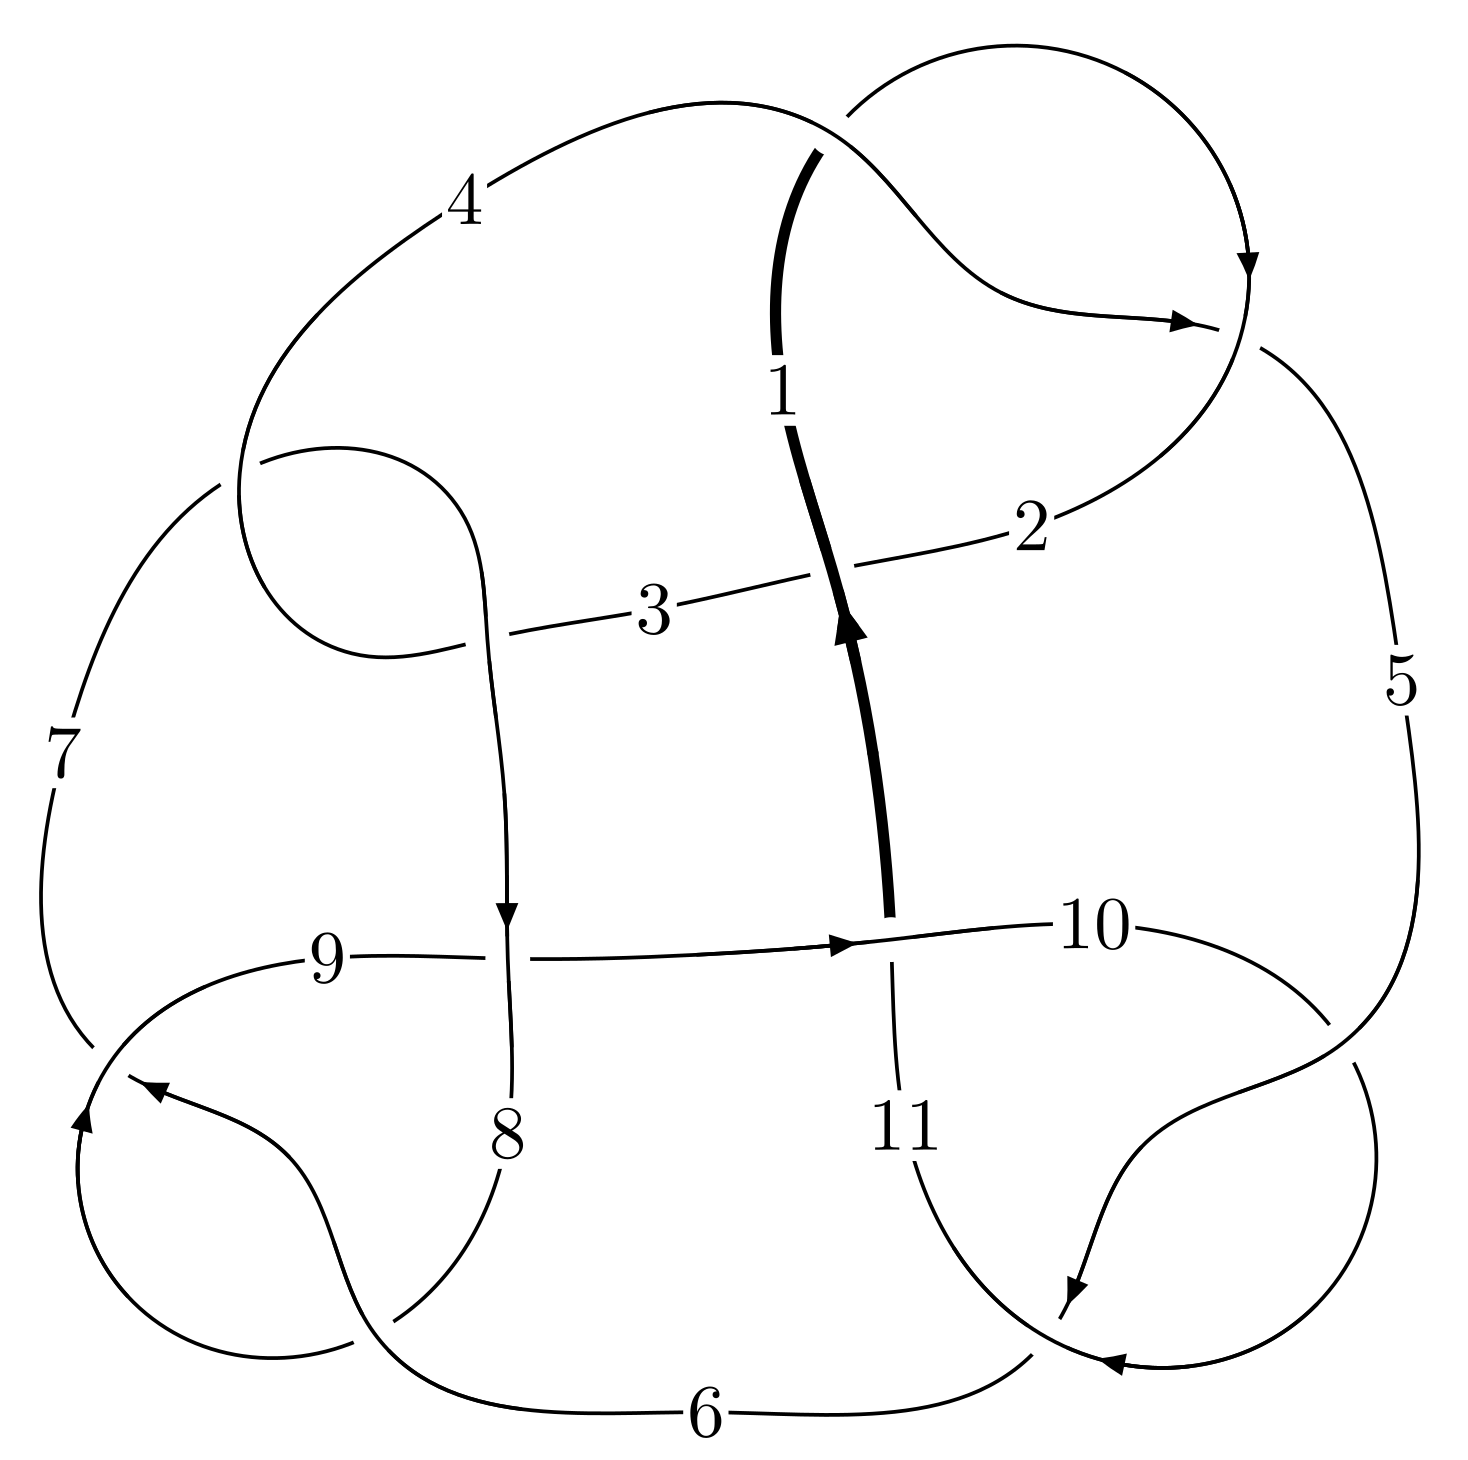
\includegraphics[width=112pt]{../../../GIT/diagram.site/Diagrams/png/688_11n_72.png}\\
\ \ \ A knot diagram\footnotemark}&
\allowdisplaybreaks
\textbf{Linearized knot diagam} \\
\cline{2-2}
 &
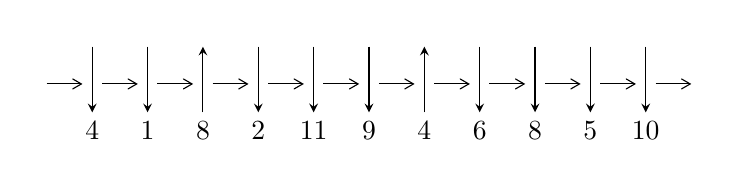
\begin{tikzpicture}[x=20pt, y=17pt]
	% nodes
	\node (C0) at (0, 0) {};
	\node (C1) at (1, 0) {};
	\node (C1U) at (1, +1) {};
	\node (C1D) at (1, -1) {4};

	\node (C2) at (2, 0) {};
	\node (C2U) at (2, +1) {};
	\node (C2D) at (2, -1) {1};

	\node (C3) at (3, 0) {};
	\node (C3U) at (3, +1) {};
	\node (C3D) at (3, -1) {8};

	\node (C4) at (4, 0) {};
	\node (C4U) at (4, +1) {};
	\node (C4D) at (4, -1) {2};

	\node (C5) at (5, 0) {};
	\node (C5U) at (5, +1) {};
	\node (C5D) at (5, -1) {11};

	\node (C6) at (6, 0) {};
	\node (C6U) at (6, +1) {};
	\node (C6D) at (6, -1) {9};

	\node (C7) at (7, 0) {};
	\node (C7U) at (7, +1) {};
	\node (C7D) at (7, -1) {4};

	\node (C8) at (8, 0) {};
	\node (C8U) at (8, +1) {};
	\node (C8D) at (8, -1) {6};

	\node (C9) at (9, 0) {};
	\node (C9U) at (9, +1) {};
	\node (C9D) at (9, -1) {8};

	\node (C10) at (10, 0) {};
	\node (C10U) at (10, +1) {};
	\node (C10D) at (10, -1) {5};

	\node (C11) at (11, 0) {};
	\node (C11U) at (11, +1) {};
	\node (C11D) at (11, -1) {10};
	\node (C12) at (12, 0) {};

	% arrows
	\draw[->,>={angle 60}]
	(C0) edge (C1) (C1) edge (C2) (C2) edge (C3) (C3) edge (C4) (C4) edge (C5) (C5) edge (C6) (C6) edge (C7) (C7) edge (C8) (C8) edge (C9) (C9) edge (C10) (C10) edge (C11) (C11) edge (C12) ;	\draw[->,>=stealth]
	(C1U) edge (C1D) (C2U) edge (C2D) (C3D) edge (C3U) (C4U) edge (C4D) (C5U) edge (C5D) (C6U) edge (C6D) (C7D) edge (C7U) (C8U) edge (C8D) (C9U) edge (C9D) (C10U) edge (C10D) (C11U) edge (C11D) ;
	\end{tikzpicture} \\
\hhline{~~} \\& 
\textbf{Solving Sequence} \\ \cline{2-2} 
 &
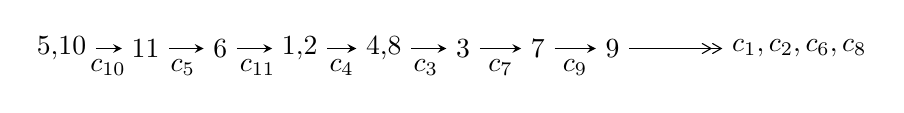
\begin{tikzpicture}[x=27pt, y=7pt]
	% node
	\node (A0) at (-1/8, 0) {5,10};
	\node (A1) at (1, 0) {11};
	\node (A2) at (2, 0) {6};
	\node (A3) at (49/16, 0) {1,2};
	\node (A4) at (67/16, 0) {4,8};
	\node (A5) at (21/4, 0) {3};
	\node (A6) at (25/4, 0) {7};
	\node (A7) at (29/4, 0) {9};
	\node (C1) at (1/2, -1) {$c_{10}$};
	\node (C2) at (3/2, -1) {$c_{5}$};
	\node (C3) at (5/2, -1) {$c_{11}$};
	\node (C4) at (29/8, -1) {$c_{4}$};
	\node (C5) at (19/4, -1) {$c_{3}$};
	\node (C6) at (23/4, -1) {$c_{7}$};
	\node (C7) at (27/4, -1) {$c_{9}$};
	\node (A8) at (39/4, 0) {$c_{1},c_{2},c_{6},c_{8}$};

	% edge
	\draw[->,>=stealth]	
	(A0) edge (A1) (A1) edge (A2) (A2) edge (A3) (A3) edge (A4) (A4) edge (A5) (A5) edge (A6) (A6) edge (A7) ;
	\draw[->>,>={angle 60}]	
	(A7) edge (A8);
\end{tikzpicture} \\ 

\end{tabular} \\

\footnotetext{
The image of knot diagram is generated by the software ``\textbf{Draw programme}" developed by Andrew Bartholomew(\url{http://www.layer8.co.uk/maths/draw/index.htm\#Running-draw}), where we modified some parts for our purpose(\url{https://github.com/CATsTAILs/LinksPainter}).
}\phantom \\ \newline 
\centering \textbf{Ideals for irreducible components\footnotemark of $X_{\text{par}}$} 
 
\begin{align*}
I^u_{1}&=\langle 
u^2+d,\;- u^6- u^5+u^3-2 u^2+2 c-2 u-1,\;- u^6- u^5+u^3-2 u^2+2 b-2 u+1,\;a-1,\\
\phantom{I^u_{1}}&\phantom{= \langle  }u^8+u^7- u^6-2 u^5+2 u^4+3 u^3+u^2-2 u+1\rangle \\
I^u_{2}&=\langle 
u^2+d,\;- u^{10}-2 u^9- u^8+2 u^7+u^6-2 u^5-4 u^4+u^2+c+u-1,\;b-1,\\
\phantom{I^u_{2}}&\phantom{= \langle  }u^{10}+2 u^9- u^8-5 u^7- u^6+6 u^5+4 u^4-4 u^3-5 u^2+a+u+4,\\
\phantom{I^u_{2}}&\phantom{= \langle  }u^{11}+2 u^{10}-4 u^8-2 u^7+4 u^6+5 u^5-2 u^4-5 u^3- u^2+3 u+1\rangle \\
I^u_{3}&=\langle 
- u^{10}- u^9+u^8+2 u^7- u^6-2 u^5+2 u^3+d- u+1,\\
\phantom{I^u_{3}}&\phantom{= \langle  }u^{10}+2 u^9- u^8-5 u^7- u^6+6 u^5+4 u^4-4 u^3-5 u^2+c+u+3,\\
\phantom{I^u_{3}}&\phantom{= \langle  }- u^{10}-2 u^9- u^8+2 u^7+u^6-2 u^5-4 u^4+u^2+b+u,\;a-1,\\
\phantom{I^u_{3}}&\phantom{= \langle  }u^{11}+2 u^{10}-4 u^8-2 u^7+4 u^6+5 u^5-2 u^4-5 u^3- u^2+3 u+1\rangle \\
I^u_{4}&=\langle 
-17 u^{10}+8 u^9+27 u^8-4 u^7-39 u^6+6 u^5+68 u^4+2 u^3-75 u^2+86 d-41 u+80,\\
\phantom{I^u_{4}}&\phantom{= \langle  }-41 u^{10}-6 u^9+55 u^8+132 u^7-3 u^6-198 u^5-180 u^4+106 u^3+325 u^2+344 c-109 u-318,\;b-1,\\
\phantom{I^u_{4}}&\phantom{= \langle  }-41 u^{10}-6 u^9+55 u^8+132 u^7-3 u^6-198 u^5-180 u^4+106 u^3+325 u^2+344 a-109 u+26,\\
\phantom{I^u_{4}}&\phantom{= \langle  }u^{11}-3 u^9-2 u^8+3 u^7+4 u^6-2 u^4- u^3+3 u^2-4\rangle \\
I^u_{5}&=\langle 
d,\;c-1,\;b-1,\;a+1,\;u+1\rangle \\
I^u_{6}&=\langle 
d+1,\;c,\;b-1,\;a,\;u-1\rangle \\
I^u_{7}&=\langle 
u^2 a+d+1,\;c+a,\;b-1,\;a^2+u^2+a- u,\;u^3- u-1\rangle \\
I^u_{8}&=\langle 
d+1,\;c b- c-1,\;a+1,\;u+1\rangle \\
\\
I^v_{1}&=\langle 
a,\;d+1,\;c+a-1,\;b-1,\;v+1\rangle \\
\end{align*}
\raggedright * 8 irreducible components of $\dim_{\mathbb{C}}=0$, with total 50 representations.\\
\raggedright * 1 irreducible components of $\dim_{\mathbb{C}}=1$ \\
\footnotetext{All coefficients of polynomials are rational numbers. But the coefficients are sometimes approximated in decimal forms when there is not enough margin.}
\newpage
\renewcommand{\arraystretch}{1}
\centering \section*{I. $I^u_{1}= \langle u^2+d,\;- u^6- u^5+\cdots+2 c-1,\;- u^6- u^5+\cdots+2 b+1,\;a-1,\;u^8+u^7+\cdots-2 u+1 \rangle$}
\flushleft \textbf{(i) Arc colorings}\\
\begin{tabular}{m{7pt} m{180pt} m{7pt} m{180pt} }
\flushright $a_{5}=$&$\begin{pmatrix}0\\u\end{pmatrix}$ \\
\flushright $a_{10}=$&$\begin{pmatrix}1\\0\end{pmatrix}$ \\
\flushright $a_{11}=$&$\begin{pmatrix}1\\u^2\end{pmatrix}$ \\
\flushright $a_{6}=$&$\begin{pmatrix}- u\\- u^3+u\end{pmatrix}$ \\
\flushright $a_{1}=$&$\begin{pmatrix}- u^2+1\\u^2\end{pmatrix}$ \\
\flushright $a_{2}=$&$\begin{pmatrix}1\\\frac{1}{2} u^6+\frac{1}{2} u^5+\cdots+u-\frac{1}{2}\end{pmatrix}$ \\
\flushright $a_{4}=$&$\begin{pmatrix}u\\\frac{1}{2} u^7+\frac{1}{2} u^6+\cdots+u^2+\frac{1}{2} u\end{pmatrix}$ \\
\flushright $a_{8}=$&$\begin{pmatrix}\frac{1}{2} u^6+\frac{1}{2} u^5+\cdots+u+\frac{1}{2}\\- u^2\end{pmatrix}$ \\
\flushright $a_{3}=$&$\begin{pmatrix}u^4- u^2+1\\\frac{1}{2} u^6+\frac{1}{2} u^5+\cdots+u-\frac{1}{2}\end{pmatrix}$ \\
\flushright $a_{7}=$&$\begin{pmatrix}\frac{1}{2} u^7+\frac{1}{2} u^6-\frac{1}{2} u^4+u^2+\frac{3}{2} u\\- u^5+u^3- u\end{pmatrix}$ \\
\flushright $a_{9}=$&$\begin{pmatrix}\frac{1}{2} u^6+\frac{1}{2} u^5-\frac{1}{2} u^3+u+\frac{1}{2}\\- u^4\end{pmatrix}$\\ \flushright $a_{9}=$&$\begin{pmatrix}\frac{1}{2} u^6+\frac{1}{2} u^5-\frac{1}{2} u^3+u+\frac{1}{2}\\- u^4\end{pmatrix}$\\&\end{tabular}
\flushleft \textbf{(ii) Obstruction class $= -1$}\\~\\
\flushleft \textbf{(iii) Cusp Shapes $= 3 u^7+6 u^6- u^5-7 u^4+3 u^3+16 u^2+7 u-9$}\\~\\
\newpage\renewcommand{\arraystretch}{1}
\flushleft \textbf{(iv) u-Polynomials at the component}\newline \\
\begin{tabular}{m{50pt}|m{274pt}}
Crossings & \hspace{64pt}u-Polynomials at each crossing \\
\hline $$\begin{aligned}c_{1},c_{4},c_{5}\\c_{6},c_{8},c_{10}\end{aligned}$$&$\begin{aligned}
&u^8- u^7- u^6+2 u^5+2 u^4-3 u^3+u^2+2 u+1
\end{aligned}$\\
\hline $$\begin{aligned}c_{2},c_{9},c_{11}\end{aligned}$$&$\begin{aligned}
&u^8+3 u^7+9 u^6+12 u^5+20 u^4+15 u^3+17 u^2+2 u+1
\end{aligned}$\\
\hline $$\begin{aligned}c_{3},c_{7}\end{aligned}$$&$\begin{aligned}
&u^8- u^7- u^6+5 u^5-4 u^4+8 u^2-4 u+4
\end{aligned}$\\
\hline
\end{tabular}\\~\\
\newpage\renewcommand{\arraystretch}{1}
\flushleft \textbf{(v) Riley Polynomials at the component}\newline \\
\begin{tabular}{m{50pt}|m{274pt}}
Crossings & \hspace{64pt}Riley Polynomials at each crossing \\
\hline $$\begin{aligned}c_{1},c_{4},c_{5}\\c_{6},c_{8},c_{10}\end{aligned}$$&$\begin{aligned}
&y^8-3 y^7+9 y^6-12 y^5+20 y^4-15 y^3+17 y^2-2 y+1
\end{aligned}$\\
\hline $$\begin{aligned}c_{2},c_{9},c_{11}\end{aligned}$$&$\begin{aligned}
&y^8+9 y^7+49 y^6+160 y^5+336 y^4+425 y^3+269 y^2+30 y+1
\end{aligned}$\\
\hline $$\begin{aligned}c_{3},c_{7}\end{aligned}$$&$\begin{aligned}
&y^8-3 y^7+3 y^6- y^5-32 y^3+32 y^2+48 y+16
\end{aligned}$\\
\hline
\end{tabular}\\~\\
\newpage\flushleft \textbf{(vi) Complex Volumes and Cusp Shapes}
$$\begin{array}{c|c|c}  
\text{Solutions to }I^u_{1}& \I (\text{vol} + \sqrt{-1}CS) & \text{Cusp shape}\\
 \hline 
\begin{aligned}
u &= -0.725725 + 0.895340 I \\
a &= \phantom{-}1.00000\phantom{ +0.000000I} \\
b &= -1.23064 - 0.78420 I \\
c &= -0.230638 - 0.784197 I \\
d &= \phantom{-}0.274957 + 1.299540 I\end{aligned}
 & \phantom{-}6.13361 + 3.53925 I & -3.48597 - 4.52491 I \\ \hline\begin{aligned}
u &= -0.725725 - 0.895340 I \\
a &= \phantom{-}1.00000\phantom{ +0.000000I} \\
b &= -1.23064 + 0.78420 I \\
c &= -0.230638 + 0.784197 I \\
d &= \phantom{-}0.274957 - 1.299540 I\end{aligned}
 & \phantom{-}6.13361 - 3.53925 I & -3.48597 + 4.52491 I \\ \hline\begin{aligned}
u &= \phantom{-}1.052770 + 0.635427 I \\
a &= \phantom{-}1.00000\phantom{ +0.000000I} \\
b &= -1.68524 + 1.42536 I \\
c &= -0.68524 + 1.42536 I \\
d &= -0.70455 - 1.33791 I\end{aligned}
 & -1.61416 - 7.63502 I & -9.74769 + 6.83193 I \\ \hline\begin{aligned}
u &= \phantom{-}1.052770 - 0.635427 I \\
a &= \phantom{-}1.00000\phantom{ +0.000000I} \\
b &= -1.68524 - 1.42536 I \\
c &= -0.68524 - 1.42536 I \\
d &= -0.70455 + 1.33791 I\end{aligned}
 & -1.61416 + 7.63502 I & -9.74769 - 6.83193 I \\ \hline\begin{aligned}
u &= -1.213440 + 0.663590 I \\
a &= \phantom{-}1.00000\phantom{ +0.000000I} \\
b &= -2.02473 - 1.24139 I \\
c &= -1.02473 - 1.24139 I \\
d &= -1.03209 + 1.61046 I\end{aligned}
 & \phantom{-}0.8567 + 14.6934 I & -9.31845 - 9.04054 I \\ \hline\begin{aligned}
u &= -1.213440 - 0.663590 I \\
a &= \phantom{-}1.00000\phantom{ +0.000000I} \\
b &= -2.02473 + 1.24139 I \\
c &= -1.02473 + 1.24139 I \\
d &= -1.03209 - 1.61046 I\end{aligned}
 & \phantom{-}0.8567 - 14.6934 I & -9.31845 + 9.04054 I\\
 \hline 
 \end{array}$$\newpage$$\begin{array}{c|c|c}  
\text{Solutions to }I^u_{1}& \I (\text{vol} + \sqrt{-1}CS) & \text{Cusp shape}\\
 \hline 
\begin{aligned}
u &= \phantom{-}0.386400 + 0.333144 I \\
a &= \phantom{-}1.00000\phantom{ +0.000000I} \\
b &= -0.059390 + 0.519525 I \\
c &= \phantom{-}0.940610 + 0.519525 I \\
d &= -0.038320 - 0.257454 I\end{aligned}
 & -0.441338 - 1.103720 I & -5.44788 + 6.54224 I \\ \hline\begin{aligned}
u &= \phantom{-}0.386400 - 0.333144 I \\
a &= \phantom{-}1.00000\phantom{ +0.000000I} \\
b &= -0.059390 - 0.519525 I \\
c &= \phantom{-}0.940610 - 0.519525 I \\
d &= -0.038320 + 0.257454 I\end{aligned}
 & -0.441338 + 1.103720 I & -5.44788 - 6.54224 I\\
 \hline 
 \end{array}$$\newpage\newpage\renewcommand{\arraystretch}{1}
\centering \section*{II. $I^u_{2}= \langle u^2+d,\;- u^{10}-2 u^9+\cdots+c-1,\;b-1,\;u^{10}+2 u^9+\cdots+a+4,\;u^{11}+2 u^{10}+\cdots+3 u+1 \rangle$}
\flushleft \textbf{(i) Arc colorings}\\
\begin{tabular}{m{7pt} m{180pt} m{7pt} m{180pt} }
\flushright $a_{5}=$&$\begin{pmatrix}0\\u\end{pmatrix}$ \\
\flushright $a_{10}=$&$\begin{pmatrix}1\\0\end{pmatrix}$ \\
\flushright $a_{11}=$&$\begin{pmatrix}1\\u^2\end{pmatrix}$ \\
\flushright $a_{6}=$&$\begin{pmatrix}- u\\- u^3+u\end{pmatrix}$ \\
\flushright $a_{1}=$&$\begin{pmatrix}- u^2+1\\u^2\end{pmatrix}$ \\
\flushright $a_{2}=$&$\begin{pmatrix}- u^{10}-2 u^9+u^8+5 u^7+u^6-6 u^5-4 u^4+4 u^3+5 u^2- u-4\\1\end{pmatrix}$ \\
\flushright $a_{4}=$&$\begin{pmatrix}- u^{10}-3 u^9- u^8+5 u^7+4 u^6-5 u^5-7 u^4+2 u^3+7 u^2+u-4\\u^9+u^8- u^7-2 u^6+u^5+2 u^4-2 u^2+1\end{pmatrix}$ \\
\flushright $a_{8}=$&$\begin{pmatrix}u^{10}+2 u^9+u^8-2 u^7- u^6+2 u^5+4 u^4- u^2- u+1\\- u^2\end{pmatrix}$ \\
\flushright $a_{3}=$&$\begin{pmatrix}- u^{10}-3 u^9+u^8+7 u^7+3 u^6-9 u^5-7 u^4+5 u^3+10 u^2-2 u-6\\u^{10}+2 u^9- u^8-4 u^7- u^6+5 u^5+3 u^4-3 u^3-5 u^2+2 u+2\end{pmatrix}$ \\
\flushright $a_{7}=$&$\begin{pmatrix}u^9+2 u^8+u^7-2 u^6- u^5+2 u^4+3 u^3- u-1\\- u^5+u^3- u\end{pmatrix}$ \\
\flushright $a_{9}=$&$\begin{pmatrix}u^{10}+2 u^9+u^8-2 u^7- u^6+2 u^5+4 u^4-2 u^2- u+1\\- u^4\end{pmatrix}$\\ \flushright $a_{9}=$&$\begin{pmatrix}u^{10}+2 u^9+u^8-2 u^7- u^6+2 u^5+4 u^4-2 u^2- u+1\\- u^4\end{pmatrix}$\\&\end{tabular}
\flushleft \textbf{(ii) Obstruction class $= -1$}\\~\\
\flushleft \textbf{(iii) Cusp Shapes $= 4 u^{10}+6 u^9-10 u^7-4 u^6+6 u^5+12 u^4-4 u^3-8 u^2-6 u-4$}\\~\\
\newpage\renewcommand{\arraystretch}{1}
\flushleft \textbf{(iv) u-Polynomials at the component}\newline \\
\begin{tabular}{m{50pt}|m{274pt}}
Crossings & \hspace{64pt}u-Polynomials at each crossing \\
\hline $$\begin{aligned}c_{1},c_{4}\end{aligned}$$&$\begin{aligned}
&u^{11}-3 u^9+2 u^8+3 u^7-4 u^6+2 u^4- u^3-3 u^2+4
\end{aligned}$\\
\hline $$\begin{aligned}c_{2}\end{aligned}$$&$\begin{aligned}
&u^{11}+6 u^{10}+\cdots+24 u+16
\end{aligned}$\\
\hline $$\begin{aligned}c_{3},c_{7}\end{aligned}$$&$\begin{aligned}
&u^{11}-2 u^{10}- u^9+3 u^8+u^7-2 u^6+4 u^5-11 u^4+9 u^3- u^2-2 u+2
\end{aligned}$\\
\hline $$\begin{aligned}c_{5},c_{6},c_{8}\\c_{10}\end{aligned}$$&$\begin{aligned}
&u^{11}-2 u^{10}+4 u^8-2 u^7-4 u^6+5 u^5+2 u^4-5 u^3+u^2+3 u-1
\end{aligned}$\\
\hline $$\begin{aligned}c_{9},c_{11}\end{aligned}$$&$\begin{aligned}
&u^{11}+4 u^{10}+\cdots+11 u+1
\end{aligned}$\\
\hline
\end{tabular}\\~\\
\newpage\renewcommand{\arraystretch}{1}
\flushleft \textbf{(v) Riley Polynomials at the component}\newline \\
\begin{tabular}{m{50pt}|m{274pt}}
Crossings & \hspace{64pt}Riley Polynomials at each crossing \\
\hline $$\begin{aligned}c_{1},c_{4}\end{aligned}$$&$\begin{aligned}
&y^{11}-6 y^{10}+\cdots+24 y-16
\end{aligned}$\\
\hline $$\begin{aligned}c_{2}\end{aligned}$$&$\begin{aligned}
&y^{11}-6 y^{10}+\cdots-224 y-256
\end{aligned}$\\
\hline $$\begin{aligned}c_{3},c_{7}\end{aligned}$$&$\begin{aligned}
&y^{11}-6 y^{10}+\cdots+8 y-4
\end{aligned}$\\
\hline $$\begin{aligned}c_{5},c_{6},c_{8}\\c_{10}\end{aligned}$$&$\begin{aligned}
&y^{11}-4 y^{10}+\cdots+11 y-1
\end{aligned}$\\
\hline $$\begin{aligned}c_{9},c_{11}\end{aligned}$$&$\begin{aligned}
&y^{11}+8 y^{10}+\cdots+67 y-1
\end{aligned}$\\
\hline
\end{tabular}\\~\\
\newpage\flushleft \textbf{(vi) Complex Volumes and Cusp Shapes}
$$\begin{array}{c|c|c}  
\text{Solutions to }I^u_{2}& \I (\text{vol} + \sqrt{-1}CS) & \text{Cusp shape}\\
 \hline 
\begin{aligned}
u &= \phantom{-}0.952018 + 0.226513 I \\
a &= -1.085970 + 0.401284 I \\
b &= \phantom{-}1.00000\phantom{ +0.000000I} \\
c &= \phantom{-}0.40050 + 4.16652 I \\
d &= -0.855030 - 0.431288 I\end{aligned}
 & -5.02081 - 0.74196 I & -15.5393 + 1.1191 I \\ \hline\begin{aligned}
u &= \phantom{-}0.952018 - 0.226513 I \\
a &= -1.085970 - 0.401284 I \\
b &= \phantom{-}1.00000\phantom{ +0.000000I} \\
c &= \phantom{-}0.40050 - 4.16652 I \\
d &= -0.855030 + 0.431288 I\end{aligned}
 & -5.02081 + 0.74196 I & -15.5393 - 1.1191 I \\ \hline\begin{aligned}
u &= \phantom{-}0.850023 + 0.614930 I \\
a &= \phantom{-}0.007368 - 0.850380 I \\
b &= \phantom{-}1.00000\phantom{ +0.000000I} \\
c &= -0.138893 + 1.373110 I \\
d &= -0.344399 - 1.045410 I\end{aligned}
 & -0.08426 - 2.41892 I & -7.07184 + 2.88947 I \\ \hline\begin{aligned}
u &= \phantom{-}0.850023 - 0.614930 I \\
a &= \phantom{-}0.007368 + 0.850380 I \\
b &= \phantom{-}1.00000\phantom{ +0.000000I} \\
c &= -0.138893 - 1.373110 I \\
d &= -0.344399 + 1.045410 I\end{aligned}
 & -0.08426 + 2.41892 I & -7.07184 - 2.88947 I \\ \hline\begin{aligned}
u &= -0.523691 + 0.948055 I \\
a &= -0.184008 + 1.141810 I \\
b &= \phantom{-}1.00000\phantom{ +0.000000I} \\
c &= -0.103739 - 0.547821 I \\
d &= \phantom{-}0.624556 + 0.992977 I\end{aligned}
 & \phantom{-}5.32590 - 2.58451 I & -3.80806 + 1.01660 I \\ \hline\begin{aligned}
u &= -0.523691 - 0.948055 I \\
a &= -0.184008 - 1.141810 I \\
b &= \phantom{-}1.00000\phantom{ +0.000000I} \\
c &= -0.103739 + 0.547821 I \\
d &= \phantom{-}0.624556 - 0.992977 I\end{aligned}
 & \phantom{-}5.32590 + 2.58451 I & -3.80806 - 1.01660 I\\
 \hline 
 \end{array}$$\newpage$$\begin{array}{c|c|c}  
\text{Solutions to }I^u_{2}& \I (\text{vol} + \sqrt{-1}CS) & \text{Cusp shape}\\
 \hline 
\begin{aligned}
u &= -0.978643 + 0.595733 I \\
a &= -0.939343 - 0.770160 I \\
b &= \phantom{-}1.00000\phantom{ +0.000000I} \\
c &= -0.47651 - 1.53693 I \\
d &= -0.602844 + 1.166020 I\end{aligned}
 & -2.61864 + 4.69742 I & -9.08124 - 5.88322 I \\ \hline\begin{aligned}
u &= -0.978643 - 0.595733 I \\
a &= -0.939343 + 0.770160 I \\
b &= \phantom{-}1.00000\phantom{ +0.000000I} \\
c &= -0.47651 + 1.53693 I \\
d &= -0.602844 - 1.166020 I\end{aligned}
 & -2.61864 - 4.69742 I & -9.08124 + 5.88322 I \\ \hline\begin{aligned}
u &= -1.126060 + 0.711355 I \\
a &= -0.175044 + 0.783251 I \\
b &= \phantom{-}1.00000\phantom{ +0.000000I} \\
c &= -0.81852 - 1.22144 I \\
d &= -0.76197 + 1.60205 I\end{aligned}
 & \phantom{-}3.47965 + 8.65115 I & -6.21430 - 5.57892 I \\ \hline\begin{aligned}
u &= -1.126060 - 0.711355 I \\
a &= -0.175044 - 0.783251 I \\
b &= \phantom{-}1.00000\phantom{ +0.000000I} \\
c &= -0.81852 + 1.22144 I \\
d &= -0.76197 - 1.60205 I\end{aligned}
 & \phantom{-}3.47965 - 8.65115 I & -6.21430 + 5.57892 I \\ \hline\begin{aligned}
u &= -0.347303\phantom{ +0.000000I} \\
a &= -3.24600\phantom{ +0.000000I} \\
b &= \phantom{-}1.00000\phantom{ +0.000000I} \\
c &= \phantom{-}1.27433\phantom{ +0.000000I} \\
d &= -0.120619\phantom{ +0.000000I}\end{aligned}
 & -2.16369\phantom{ +0.000000I} & -2.57060\phantom{ +0.000000I}\\
 \hline 
 \end{array}$$\newpage\newpage\renewcommand{\arraystretch}{1}
\centering \section*{III. $I^u_{3}= \langle - u^{10}- u^9+\cdots+d+1,\;u^{10}+2 u^9+\cdots+c+3,\;- u^{10}-2 u^9+\cdots+b+u,\;a-1,\;u^{11}+2 u^{10}+\cdots+3 u+1 \rangle$}
\flushleft \textbf{(i) Arc colorings}\\
\begin{tabular}{m{7pt} m{180pt} m{7pt} m{180pt} }
\flushright $a_{5}=$&$\begin{pmatrix}0\\u\end{pmatrix}$ \\
\flushright $a_{10}=$&$\begin{pmatrix}1\\0\end{pmatrix}$ \\
\flushright $a_{11}=$&$\begin{pmatrix}1\\u^2\end{pmatrix}$ \\
\flushright $a_{6}=$&$\begin{pmatrix}- u\\- u^3+u\end{pmatrix}$ \\
\flushright $a_{1}=$&$\begin{pmatrix}- u^2+1\\u^2\end{pmatrix}$ \\
\flushright $a_{2}=$&$\begin{pmatrix}1\\u^{10}+2 u^9+u^8-2 u^7- u^6+2 u^5+4 u^4- u^2- u\end{pmatrix}$ \\
\flushright $a_{4}=$&$\begin{pmatrix}u\\u^9+2 u^8+u^7-2 u^6- u^5+2 u^4+4 u^3-2 u-1\end{pmatrix}$ \\
\flushright $a_{8}=$&$\begin{pmatrix}- u^{10}-2 u^9+u^8+5 u^7+u^6-6 u^5-4 u^4+4 u^3+5 u^2- u-3\\u^{10}+u^9- u^8-2 u^7+u^6+2 u^5-2 u^3+u-1\end{pmatrix}$ \\
\flushright $a_{3}=$&$\begin{pmatrix}u^4- u^2+1\\u^{10}+2 u^9+u^8-2 u^7- u^6+2 u^5+3 u^4- u^2- u\end{pmatrix}$ \\
\flushright $a_{7}=$&$\begin{pmatrix}-2 u^{10}-3 u^9+2 u^8+7 u^7-9 u^5-5 u^4+7 u^3+7 u^2-3 u-4\\u^{10}- u^9-3 u^8- u^7+5 u^6+2 u^5-3 u^4-5 u^3+3 u^2+3 u-1\end{pmatrix}$ \\
\flushright $a_{9}=$&$\begin{pmatrix}-2 u^{10}-3 u^9+2 u^8+7 u^7-8 u^5-4 u^4+6 u^3+6 u^2-2 u-3\\u^{10}- u^8+3 u^6- u^5-2 u^4- u^3+3 u^2-2\end{pmatrix}$\\ \flushright $a_{9}=$&$\begin{pmatrix}-2 u^{10}-3 u^9+2 u^8+7 u^7-8 u^5-4 u^4+6 u^3+6 u^2-2 u-3\\u^{10}- u^8+3 u^6- u^5-2 u^4- u^3+3 u^2-2\end{pmatrix}$\\&\end{tabular}
\flushleft \textbf{(ii) Obstruction class $= -1$}\\~\\
\flushleft \textbf{(iii) Cusp Shapes $= 4 u^{10}+6 u^9-10 u^7-4 u^6+6 u^5+12 u^4-4 u^3-8 u^2-6 u-4$}\\~\\
\newpage\renewcommand{\arraystretch}{1}
\flushleft \textbf{(iv) u-Polynomials at the component}\newline \\
\begin{tabular}{m{50pt}|m{274pt}}
Crossings & \hspace{64pt}u-Polynomials at each crossing \\
\hline $$\begin{aligned}c_{1},c_{4},c_{5}\\c_{10}\end{aligned}$$&$\begin{aligned}
&u^{11}-2 u^{10}+4 u^8-2 u^7-4 u^6+5 u^5+2 u^4-5 u^3+u^2+3 u-1
\end{aligned}$\\
\hline $$\begin{aligned}c_{2},c_{11}\end{aligned}$$&$\begin{aligned}
&u^{11}+4 u^{10}+\cdots+11 u+1
\end{aligned}$\\
\hline $$\begin{aligned}c_{3},c_{7}\end{aligned}$$&$\begin{aligned}
&u^{11}-2 u^{10}- u^9+3 u^8+u^7-2 u^6+4 u^5-11 u^4+9 u^3- u^2-2 u+2
\end{aligned}$\\
\hline $$\begin{aligned}c_{6},c_{8}\end{aligned}$$&$\begin{aligned}
&u^{11}-3 u^9+2 u^8+3 u^7-4 u^6+2 u^4- u^3-3 u^2+4
\end{aligned}$\\
\hline $$\begin{aligned}c_{9}\end{aligned}$$&$\begin{aligned}
&u^{11}+6 u^{10}+\cdots+24 u+16
\end{aligned}$\\
\hline
\end{tabular}\\~\\
\newpage\renewcommand{\arraystretch}{1}
\flushleft \textbf{(v) Riley Polynomials at the component}\newline \\
\begin{tabular}{m{50pt}|m{274pt}}
Crossings & \hspace{64pt}Riley Polynomials at each crossing \\
\hline $$\begin{aligned}c_{1},c_{4},c_{5}\\c_{10}\end{aligned}$$&$\begin{aligned}
&y^{11}-4 y^{10}+\cdots+11 y-1
\end{aligned}$\\
\hline $$\begin{aligned}c_{2},c_{11}\end{aligned}$$&$\begin{aligned}
&y^{11}+8 y^{10}+\cdots+67 y-1
\end{aligned}$\\
\hline $$\begin{aligned}c_{3},c_{7}\end{aligned}$$&$\begin{aligned}
&y^{11}-6 y^{10}+\cdots+8 y-4
\end{aligned}$\\
\hline $$\begin{aligned}c_{6},c_{8}\end{aligned}$$&$\begin{aligned}
&y^{11}-6 y^{10}+\cdots+24 y-16
\end{aligned}$\\
\hline $$\begin{aligned}c_{9}\end{aligned}$$&$\begin{aligned}
&y^{11}-6 y^{10}+\cdots-224 y-256
\end{aligned}$\\
\hline
\end{tabular}\\~\\
\newpage\flushleft \textbf{(vi) Complex Volumes and Cusp Shapes}
$$\begin{array}{c|c|c}  
\text{Solutions to }I^u_{3}& \I (\text{vol} + \sqrt{-1}CS) & \text{Cusp shape}\\
 \hline 
\begin{aligned}
u &= \phantom{-}0.952018 + 0.226513 I \\
a &= \phantom{-}1.00000\phantom{ +0.000000I} \\
b &= -0.59950 + 4.16652 I \\
c &= -0.085971 + 0.401284 I \\
d &= -1.246580 + 0.306031 I\end{aligned}
 & -5.02081 - 0.74196 I & -15.5393 + 1.1191 I \\ \hline\begin{aligned}
u &= \phantom{-}0.952018 - 0.226513 I \\
a &= \phantom{-}1.00000\phantom{ +0.000000I} \\
b &= -0.59950 - 4.16652 I \\
c &= -0.085971 - 0.401284 I \\
d &= -1.246580 - 0.306031 I\end{aligned}
 & -5.02081 + 0.74196 I & -15.5393 - 1.1191 I \\ \hline\begin{aligned}
u &= \phantom{-}0.850023 + 0.614930 I \\
a &= \phantom{-}1.00000\phantom{ +0.000000I} \\
b &= -1.13889 + 1.37311 I \\
c &= \phantom{-}1.007370 - 0.850380 I \\
d &= \phantom{-}0.235931 + 0.760242 I\end{aligned}
 & -0.08426 - 2.41892 I & -7.07184 + 2.88947 I \\ \hline\begin{aligned}
u &= \phantom{-}0.850023 - 0.614930 I \\
a &= \phantom{-}1.00000\phantom{ +0.000000I} \\
b &= -1.13889 - 1.37311 I \\
c &= \phantom{-}1.007370 + 0.850380 I \\
d &= \phantom{-}0.235931 - 0.760242 I\end{aligned}
 & -0.08426 + 2.41892 I & -7.07184 - 2.88947 I \\ \hline\begin{aligned}
u &= -0.523691 + 0.948055 I \\
a &= \phantom{-}1.00000\phantom{ +0.000000I} \\
b &= -1.103740 - 0.547821 I \\
c &= \phantom{-}0.815992 + 1.141810 I \\
d &= -0.37585 - 1.52338 I\end{aligned}
 & \phantom{-}5.32590 - 2.58451 I & -3.80806 + 1.01660 I \\ \hline\begin{aligned}
u &= -0.523691 - 0.948055 I \\
a &= \phantom{-}1.00000\phantom{ +0.000000I} \\
b &= -1.103740 + 0.547821 I \\
c &= \phantom{-}0.815992 - 1.141810 I \\
d &= -0.37585 + 1.52338 I\end{aligned}
 & \phantom{-}5.32590 + 2.58451 I & -3.80806 - 1.01660 I\\
 \hline 
 \end{array}$$\newpage$$\begin{array}{c|c|c}  
\text{Solutions to }I^u_{3}& \I (\text{vol} + \sqrt{-1}CS) & \text{Cusp shape}\\
 \hline 
\begin{aligned}
u &= -0.978643 + 0.595733 I \\
a &= \phantom{-}1.00000\phantom{ +0.000000I} \\
b &= -1.47651 - 1.53693 I \\
c &= \phantom{-}0.060657 - 0.770160 I \\
d &= -1.86145 - 0.53501 I\end{aligned}
 & -2.61864 + 4.69742 I & -9.08124 - 5.88322 I \\ \hline\begin{aligned}
u &= -0.978643 - 0.595733 I \\
a &= \phantom{-}1.00000\phantom{ +0.000000I} \\
b &= -1.47651 + 1.53693 I \\
c &= \phantom{-}0.060657 + 0.770160 I \\
d &= -1.86145 + 0.53501 I\end{aligned}
 & -2.61864 - 4.69742 I & -9.08124 + 5.88322 I \\ \hline\begin{aligned}
u &= -1.126060 + 0.711355 I \\
a &= \phantom{-}1.00000\phantom{ +0.000000I} \\
b &= -1.81852 - 1.22144 I \\
c &= \phantom{-}0.824956 + 0.783251 I \\
d &= \phantom{-}0.883402 - 0.724805 I\end{aligned}
 & \phantom{-}3.47965 + 8.65115 I & -6.21430 - 5.57892 I \\ \hline\begin{aligned}
u &= -1.126060 - 0.711355 I \\
a &= \phantom{-}1.00000\phantom{ +0.000000I} \\
b &= -1.81852 + 1.22144 I \\
c &= \phantom{-}0.824956 - 0.783251 I \\
d &= \phantom{-}0.883402 + 0.724805 I\end{aligned}
 & \phantom{-}3.47965 - 8.65115 I & -6.21430 + 5.57892 I \\ \hline\begin{aligned}
u &= -0.347303\phantom{ +0.000000I} \\
a &= \phantom{-}1.00000\phantom{ +0.000000I} \\
b &= \phantom{-}0.274328\phantom{ +0.000000I} \\
c &= -2.24600\phantom{ +0.000000I} \\
d &= -1.27091\phantom{ +0.000000I}\end{aligned}
 & -2.16369\phantom{ +0.000000I} & -2.57060\phantom{ +0.000000I}\\
 \hline 
 \end{array}$$\newpage\newpage\renewcommand{\arraystretch}{1}
\centering \section*{IV. $I^u_{4}= \langle -17 u^{10}+8 u^9+\cdots+86 d+80,\;-41 u^{10}-6 u^{9}+\cdots+344 c-318,\;b-1,\;-41 u^{10}-6 u^{9}+\cdots+344 a+26,\;u^{11}-3 u^9+\cdots+3 u^2-4 \rangle$}
\flushleft \textbf{(i) Arc colorings}\\
\begin{tabular}{m{7pt} m{180pt} m{7pt} m{180pt} }
\flushright $a_{5}=$&$\begin{pmatrix}0\\u\end{pmatrix}$ \\
\flushright $a_{10}=$&$\begin{pmatrix}1\\0\end{pmatrix}$ \\
\flushright $a_{11}=$&$\begin{pmatrix}1\\u^2\end{pmatrix}$ \\
\flushright $a_{6}=$&$\begin{pmatrix}- u\\- u^3+u\end{pmatrix}$ \\
\flushright $a_{1}=$&$\begin{pmatrix}- u^2+1\\u^2\end{pmatrix}$ \\
\flushright $a_{2}=$&$\begin{pmatrix}0.119186 u^{10}+0.0174419 u^{9}+\cdots+0.316860 u-0.0755814\\1\end{pmatrix}$ \\
\flushright $a_{4}=$&$\begin{pmatrix}0.232558 u^{10}-0.197674 u^{9}+\cdots-0.174419 u-0.476744\\0.0174419 u^{10}+0.197674 u^{9}+\cdots+0.924419 u+0.476744\end{pmatrix}$ \\
\flushright $a_{8}=$&$\begin{pmatrix}0.119186 u^{10}+0.0174419 u^{9}+\cdots+0.316860 u+0.924419\\0.197674 u^{10}-0.0930233 u^{9}+\cdots+0.476744 u-0.930233\end{pmatrix}$ \\
\flushright $a_{3}=$&$\begin{pmatrix}0.0377907 u^{10}-0.238372 u^{9}+\cdots+0.00290698 u-0.633721\\0.279070 u^{10}+0.162791 u^{9}+\cdots+0.790698 u+0.627907\end{pmatrix}$ \\
\flushright $a_{7}=$&$\begin{pmatrix}0.156977 u^{10}+0.279070 u^{9}+\cdots-0.180233 u+0.790698\\0.238372 u^{10}+0.0348837 u^{9}+\cdots+0.633721 u-0.151163\end{pmatrix}$ \\
\flushright $a_{9}=$&$\begin{pmatrix}-0.0784884 u^{10}+0.110465 u^{9}+\cdots-0.159884 u+0.854651\\0.116279 u^{10}-0.348837 u^{9}+\cdots+0.162791 u-0.488372\end{pmatrix}$\\ \flushright $a_{9}=$&$\begin{pmatrix}-0.0784884 u^{10}+0.110465 u^{9}+\cdots-0.159884 u+0.854651\\0.116279 u^{10}-0.348837 u^{9}+\cdots+0.162791 u-0.488372\end{pmatrix}$\\&\end{tabular}
\flushleft \textbf{(ii) Obstruction class $= -1$}\\~\\
\flushleft \textbf{(iii) Cusp Shapes $= \frac{54}{43} u^{10}+\frac{10}{43} u^9-\frac{106}{43} u^8-\frac{134}{43} u^7-\frac{38}{43} u^6+\frac{158}{43} u^5+\frac{128}{43} u^4+\frac{24}{43} u^3-\frac{126}{43} u^2+\frac{196}{43} u-\frac{244}{43}$}\\~\\
\newpage\renewcommand{\arraystretch}{1}
\flushleft \textbf{(iv) u-Polynomials at the component}\newline \\
\begin{tabular}{m{50pt}|m{274pt}}
Crossings & \hspace{64pt}u-Polynomials at each crossing \\
\hline $$\begin{aligned}c_{1},c_{4},c_{6}\\c_{8}\end{aligned}$$&$\begin{aligned}
&u^{11}-2 u^{10}+4 u^8-2 u^7-4 u^6+5 u^5+2 u^4-5 u^3+u^2+3 u-1
\end{aligned}$\\
\hline $$\begin{aligned}c_{2},c_{9}\end{aligned}$$&$\begin{aligned}
&u^{11}+4 u^{10}+\cdots+11 u+1
\end{aligned}$\\
\hline $$\begin{aligned}c_{3},c_{7}\end{aligned}$$&$\begin{aligned}
&u^{11}-2 u^{10}- u^9+3 u^8+u^7-2 u^6+4 u^5-11 u^4+9 u^3- u^2-2 u+2
\end{aligned}$\\
\hline $$\begin{aligned}c_{5},c_{10}\end{aligned}$$&$\begin{aligned}
&u^{11}-3 u^9+2 u^8+3 u^7-4 u^6+2 u^4- u^3-3 u^2+4
\end{aligned}$\\
\hline $$\begin{aligned}c_{11}\end{aligned}$$&$\begin{aligned}
&u^{11}+6 u^{10}+\cdots+24 u+16
\end{aligned}$\\
\hline
\end{tabular}\\~\\
\newpage\renewcommand{\arraystretch}{1}
\flushleft \textbf{(v) Riley Polynomials at the component}\newline \\
\begin{tabular}{m{50pt}|m{274pt}}
Crossings & \hspace{64pt}Riley Polynomials at each crossing \\
\hline $$\begin{aligned}c_{1},c_{4},c_{6}\\c_{8}\end{aligned}$$&$\begin{aligned}
&y^{11}-4 y^{10}+\cdots+11 y-1
\end{aligned}$\\
\hline $$\begin{aligned}c_{2},c_{9}\end{aligned}$$&$\begin{aligned}
&y^{11}+8 y^{10}+\cdots+67 y-1
\end{aligned}$\\
\hline $$\begin{aligned}c_{3},c_{7}\end{aligned}$$&$\begin{aligned}
&y^{11}-6 y^{10}+\cdots+8 y-4
\end{aligned}$\\
\hline $$\begin{aligned}c_{5},c_{10}\end{aligned}$$&$\begin{aligned}
&y^{11}-6 y^{10}+\cdots+24 y-16
\end{aligned}$\\
\hline $$\begin{aligned}c_{11}\end{aligned}$$&$\begin{aligned}
&y^{11}-6 y^{10}+\cdots-224 y-256
\end{aligned}$\\
\hline
\end{tabular}\\~\\
\newpage\flushleft \textbf{(vi) Complex Volumes and Cusp Shapes}
$$\begin{array}{c|c|c}  
\text{Solutions to }I^u_{4}& \I (\text{vol} + \sqrt{-1}CS) & \text{Cusp shape}\\
 \hline 
\begin{aligned}
u &= -0.360061 + 1.006500 I \\
a &= -0.271755 + 1.216000 I \\
b &= \phantom{-}1.00000\phantom{ +0.000000I} \\
c &= \phantom{-}0.72825 + 1.21600 I \\
d &= -0.76197 - 1.60205 I\end{aligned}
 & \phantom{-}3.47965 - 8.65115 I & -6.21430 + 5.57892 I \\ \hline\begin{aligned}
u &= -0.360061 - 1.006500 I \\
a &= -0.271755 - 1.216000 I \\
b &= \phantom{-}1.00000\phantom{ +0.000000I} \\
c &= \phantom{-}0.72825 - 1.21600 I \\
d &= -0.76197 + 1.60205 I\end{aligned}
 & \phantom{-}3.47965 + 8.65115 I & -6.21430 - 5.57892 I \\ \hline\begin{aligned}
u &= \phantom{-}0.529187 + 0.718311 I \\
a &= \phantom{-}0.010188 - 1.175860 I \\
b &= \phantom{-}1.00000\phantom{ +0.000000I} \\
c &= \phantom{-}1.01019 - 1.17586 I \\
d &= -0.344399 + 1.045410 I\end{aligned}
 & -0.08426 + 2.41892 I & -7.07184 - 2.88947 I \\ \hline\begin{aligned}
u &= \phantom{-}0.529187 - 0.718311 I \\
a &= \phantom{-}0.010188 + 1.175860 I \\
b &= \phantom{-}1.00000\phantom{ +0.000000I} \\
c &= \phantom{-}1.01019 + 1.17586 I \\
d &= -0.344399 - 1.045410 I\end{aligned}
 & -0.08426 - 2.41892 I & -7.07184 + 2.88947 I \\ \hline\begin{aligned}
u &= \phantom{-}1.12735\phantom{ +0.000000I} \\
a &= -0.308071\phantom{ +0.000000I} \\
b &= \phantom{-}1.00000\phantom{ +0.000000I} \\
c &= \phantom{-}0.691929\phantom{ +0.000000I} \\
d &= -0.120619\phantom{ +0.000000I}\end{aligned}
 & -2.16369\phantom{ +0.000000I} & -2.57060\phantom{ +0.000000I} \\ \hline\begin{aligned}
u &= -1.124760 + 0.136043 I \\
a &= -0.810207 - 0.299385 I \\
b &= \phantom{-}1.00000\phantom{ +0.000000I} \\
c &= \phantom{-}0.189793 - 0.299385 I \\
d &= -0.855030 - 0.431288 I\end{aligned}
 & -5.02081 - 0.74196 I & -15.5393 + 1.1191 I\\
 \hline 
 \end{array}$$\newpage$$\begin{array}{c|c|c}  
\text{Solutions to }I^u_{4}& \I (\text{vol} + \sqrt{-1}CS) & \text{Cusp shape}\\
 \hline 
\begin{aligned}
u &= -1.124760 - 0.136043 I \\
a &= -0.810207 + 0.299385 I \\
b &= \phantom{-}1.00000\phantom{ +0.000000I} \\
c &= \phantom{-}0.189793 + 0.299385 I \\
d &= -0.855030 + 0.431288 I\end{aligned}
 & -5.02081 + 0.74196 I & -15.5393 - 1.1191 I \\ \hline\begin{aligned}
u &= -0.986131 + 0.772404 I \\
a &= -0.137568 + 0.853636 I \\
b &= \phantom{-}1.00000\phantom{ +0.000000I} \\
c &= \phantom{-}0.862432 + 0.853636 I \\
d &= \phantom{-}0.624556 - 0.992977 I\end{aligned}
 & \phantom{-}5.32590 + 2.58451 I & -3.80806 - 1.01660 I \\ \hline\begin{aligned}
u &= -0.986131 - 0.772404 I \\
a &= -0.137568 - 0.853636 I \\
b &= \phantom{-}1.00000\phantom{ +0.000000I} \\
c &= \phantom{-}0.862432 - 0.853636 I \\
d &= \phantom{-}0.624556 + 0.992977 I\end{aligned}
 & \phantom{-}5.32590 - 2.58451 I & -3.80806 + 1.01660 I \\ \hline\begin{aligned}
u &= \phantom{-}1.378090 + 0.194114 I \\
a &= -0.636622 + 0.521961 I \\
b &= \phantom{-}1.00000\phantom{ +0.000000I} \\
c &= \phantom{-}0.363378 + 0.521961 I \\
d &= -0.602844 + 1.166020 I\end{aligned}
 & -2.61864 + 4.69742 I & -9.08124 - 5.88322 I \\ \hline\begin{aligned}
u &= \phantom{-}1.378090 - 0.194114 I \\
a &= -0.636622 - 0.521961 I \\
b &= \phantom{-}1.00000\phantom{ +0.000000I} \\
c &= \phantom{-}0.363378 - 0.521961 I \\
d &= -0.602844 - 1.166020 I\end{aligned}
 & -2.61864 - 4.69742 I & -9.08124 + 5.88322 I\\
 \hline 
 \end{array}$$\newpage\newpage\renewcommand{\arraystretch}{1}
\centering \section*{V. $I^u_{5}= \langle d,\;c-1,\;b-1,\;a+1,\;u+1 \rangle$}
\flushleft \textbf{(i) Arc colorings}\\
\begin{tabular}{m{7pt} m{180pt} m{7pt} m{180pt} }
\flushright $a_{5}=$&$\begin{pmatrix}0\\-1\end{pmatrix}$ \\
\flushright $a_{10}=$&$\begin{pmatrix}1\\0\end{pmatrix}$ \\
\flushright $a_{11}=$&$\begin{pmatrix}1\\1\end{pmatrix}$ \\
\flushright $a_{6}=$&$\begin{pmatrix}1\\0\end{pmatrix}$ \\
\flushright $a_{1}=$&$\begin{pmatrix}0\\1\end{pmatrix}$ \\
\flushright $a_{2}=$&$\begin{pmatrix}-1\\1\end{pmatrix}$ \\
\flushright $a_{4}=$&$\begin{pmatrix}-1\\0\end{pmatrix}$ \\
\flushright $a_{8}=$&$\begin{pmatrix}1\\0\end{pmatrix}$ \\
\flushright $a_{3}=$&$\begin{pmatrix}-1\\0\end{pmatrix}$ \\
\flushright $a_{7}=$&$\begin{pmatrix}1\\0\end{pmatrix}$ \\
\flushright $a_{9}=$&$\begin{pmatrix}1\\0\end{pmatrix}$\\ \flushright $a_{9}=$&$\begin{pmatrix}1\\0\end{pmatrix}$\\&\end{tabular}
\flushleft \textbf{(ii) Obstruction class $= 1$}\\~\\
\flushleft \textbf{(iii) Cusp Shapes $= -12$}\\~\\
\newpage\renewcommand{\arraystretch}{1}
\flushleft \textbf{(iv) u-Polynomials at the component}\newline \\
\begin{tabular}{m{50pt}|m{274pt}}
Crossings & \hspace{64pt}u-Polynomials at each crossing \\
\hline $$\begin{aligned}c_{1},c_{5}\end{aligned}$$&$\begin{aligned}
&u-1
\end{aligned}$\\
\hline $$\begin{aligned}c_{2},c_{4},c_{10}\\c_{11}\end{aligned}$$&$\begin{aligned}
&u+1
\end{aligned}$\\
\hline $$\begin{aligned}c_{3},c_{6},c_{7}\\c_{8},c_{9}\end{aligned}$$&$\begin{aligned}
&u
\end{aligned}$\\
\hline
\end{tabular}\\~\\
\newpage\renewcommand{\arraystretch}{1}
\flushleft \textbf{(v) Riley Polynomials at the component}\newline \\
\begin{tabular}{m{50pt}|m{274pt}}
Crossings & \hspace{64pt}Riley Polynomials at each crossing \\
\hline $$\begin{aligned}c_{1},c_{2},c_{4}\\c_{5},c_{10},c_{11}\end{aligned}$$&$\begin{aligned}
&y-1
\end{aligned}$\\
\hline $$\begin{aligned}c_{3},c_{6},c_{7}\\c_{8},c_{9}\end{aligned}$$&$\begin{aligned}
&y
\end{aligned}$\\
\hline
\end{tabular}\\~\\
\newpage\flushleft \textbf{(vi) Complex Volumes and Cusp Shapes}
$$\begin{array}{c|c|c}  
\text{Solutions to }I^u_{5}& \I (\text{vol} + \sqrt{-1}CS) & \text{Cusp shape}\\
 \hline 
\begin{aligned}
u &= -1.00000\phantom{ +0.000000I} \\
a &= -1.00000\phantom{ +0.000000I} \\
b &= \phantom{-}1.00000\phantom{ +0.000000I} \\
c &= \phantom{-}1.00000\phantom{ +0.000000I} \\
d &= \phantom{-0.000000 } 0\end{aligned}
 & -3.28987\phantom{ +0.000000I} & -12.0000\phantom{ +0.000000I}\\
 \hline 
 \end{array}$$\newpage\newpage\renewcommand{\arraystretch}{1}
\centering \section*{VI. $I^u_{6}= \langle d+1,\;c,\;b-1,\;a,\;u-1 \rangle$}
\flushleft \textbf{(i) Arc colorings}\\
\begin{tabular}{m{7pt} m{180pt} m{7pt} m{180pt} }
\flushright $a_{5}=$&$\begin{pmatrix}0\\1\end{pmatrix}$ \\
\flushright $a_{10}=$&$\begin{pmatrix}1\\0\end{pmatrix}$ \\
\flushright $a_{11}=$&$\begin{pmatrix}1\\1\end{pmatrix}$ \\
\flushright $a_{6}=$&$\begin{pmatrix}-1\\0\end{pmatrix}$ \\
\flushright $a_{1}=$&$\begin{pmatrix}0\\1\end{pmatrix}$ \\
\flushright $a_{2}=$&$\begin{pmatrix}0\\1\end{pmatrix}$ \\
\flushright $a_{4}=$&$\begin{pmatrix}0\\1\end{pmatrix}$ \\
\flushright $a_{8}=$&$\begin{pmatrix}0\\-1\end{pmatrix}$ \\
\flushright $a_{3}=$&$\begin{pmatrix}0\\1\end{pmatrix}$ \\
\flushright $a_{7}=$&$\begin{pmatrix}0\\-1\end{pmatrix}$ \\
\flushright $a_{9}=$&$\begin{pmatrix}1\\-1\end{pmatrix}$\\ \flushright $a_{9}=$&$\begin{pmatrix}1\\-1\end{pmatrix}$\\&\end{tabular}
\flushleft \textbf{(ii) Obstruction class $= 1$}\\~\\
\flushleft \textbf{(iii) Cusp Shapes $= -12$}\\~\\
\newpage\renewcommand{\arraystretch}{1}
\flushleft \textbf{(iv) u-Polynomials at the component}\newline \\
\begin{tabular}{m{50pt}|m{274pt}}
Crossings & \hspace{64pt}u-Polynomials at each crossing \\
\hline $$\begin{aligned}c_{1},c_{2},c_{3}\\c_{4},c_{7}\end{aligned}$$&$\begin{aligned}
&u
\end{aligned}$\\
\hline $$\begin{aligned}c_{5},c_{8},c_{9}\\c_{11}\end{aligned}$$&$\begin{aligned}
&u+1
\end{aligned}$\\
\hline $$\begin{aligned}c_{6},c_{10}\end{aligned}$$&$\begin{aligned}
&u-1
\end{aligned}$\\
\hline
\end{tabular}\\~\\
\newpage\renewcommand{\arraystretch}{1}
\flushleft \textbf{(v) Riley Polynomials at the component}\newline \\
\begin{tabular}{m{50pt}|m{274pt}}
Crossings & \hspace{64pt}Riley Polynomials at each crossing \\
\hline $$\begin{aligned}c_{1},c_{2},c_{3}\\c_{4},c_{7}\end{aligned}$$&$\begin{aligned}
&y
\end{aligned}$\\
\hline $$\begin{aligned}c_{5},c_{6},c_{8}\\c_{9},c_{10},c_{11}\end{aligned}$$&$\begin{aligned}
&y-1
\end{aligned}$\\
\hline
\end{tabular}\\~\\
\newpage\flushleft \textbf{(vi) Complex Volumes and Cusp Shapes}
$$\begin{array}{c|c|c}  
\text{Solutions to }I^u_{6}& \I (\text{vol} + \sqrt{-1}CS) & \text{Cusp shape}\\
 \hline 
\begin{aligned}
u &= \phantom{-}1.00000\phantom{ +0.000000I} \\
a &= \phantom{-0.000000 } 0 \\
b &= \phantom{-}1.00000\phantom{ +0.000000I} \\
c &= \phantom{-0.000000 } 0 \\
d &= -1.00000\phantom{ +0.000000I}\end{aligned}
 & -3.28987\phantom{ +0.000000I} & -12.0000\phantom{ +0.000000I}\\
 \hline 
 \end{array}$$\newpage\newpage\renewcommand{\arraystretch}{1}
\centering \section*{VII. $I^u_{7}= \langle u^2 a+d+1,\;c+a,\;b-1,\;a^2+u^2+a- u,\;u^3- u-1 \rangle$}
\flushleft \textbf{(i) Arc colorings}\\
\begin{tabular}{m{7pt} m{180pt} m{7pt} m{180pt} }
\flushright $a_{5}=$&$\begin{pmatrix}0\\u\end{pmatrix}$ \\
\flushright $a_{10}=$&$\begin{pmatrix}1\\0\end{pmatrix}$ \\
\flushright $a_{11}=$&$\begin{pmatrix}1\\u^2\end{pmatrix}$ \\
\flushright $a_{6}=$&$\begin{pmatrix}- u\\-1\end{pmatrix}$ \\
\flushright $a_{1}=$&$\begin{pmatrix}- u^2+1\\u^2\end{pmatrix}$ \\
\flushright $a_{2}=$&$\begin{pmatrix}a\\1\end{pmatrix}$ \\
\flushright $a_{4}=$&$\begin{pmatrix}- a u+u^2- u-1\\a u+u\end{pmatrix}$ \\
\flushright $a_{8}=$&$\begin{pmatrix}- a\\- u^2 a-1\end{pmatrix}$ \\
\flushright $a_{3}=$&$\begin{pmatrix}- a u+u^2+a- u-1\\u^2 a+a u+u+1\end{pmatrix}$ \\
\flushright $a_{7}=$&$\begin{pmatrix}- a u+u^2- a- u-1\\- u^2 a+a u+u-1\end{pmatrix}$ \\
\flushright $a_{9}=$&$\begin{pmatrix}u^2 a+u^2- a\\- u^2 a+a u+u-1\end{pmatrix}$\\ \flushright $a_{9}=$&$\begin{pmatrix}u^2 a+u^2- a\\- u^2 a+a u+u-1\end{pmatrix}$\\&\end{tabular}
\flushleft \textbf{(ii) Obstruction class $= -1$}\\~\\
\flushleft \textbf{(iii) Cusp Shapes $= -6$}\\~\\
\newpage\renewcommand{\arraystretch}{1}
\flushleft \textbf{(iv) u-Polynomials at the component}\newline \\
\begin{tabular}{m{50pt}|m{274pt}}
Crossings & \hspace{64pt}u-Polynomials at each crossing \\
\hline $$\begin{aligned}c_{1},c_{4},c_{5}\\c_{6},c_{8},c_{10}\end{aligned}$$&$\begin{aligned}
&(u^3- u+1)^2
\end{aligned}$\\
\hline $$\begin{aligned}c_{2},c_{9},c_{11}\end{aligned}$$&$\begin{aligned}
&(u^3+2 u^2+u+1)^2
\end{aligned}$\\
\hline $$\begin{aligned}c_{3},c_{7}\end{aligned}$$&$\begin{aligned}
&(u+1)^6
\end{aligned}$\\
\hline
\end{tabular}\\~\\
\newpage\renewcommand{\arraystretch}{1}
\flushleft \textbf{(v) Riley Polynomials at the component}\newline \\
\begin{tabular}{m{50pt}|m{274pt}}
Crossings & \hspace{64pt}Riley Polynomials at each crossing \\
\hline $$\begin{aligned}c_{1},c_{4},c_{5}\\c_{6},c_{8},c_{10}\end{aligned}$$&$\begin{aligned}
&(y^3-2 y^2+y-1)^2
\end{aligned}$\\
\hline $$\begin{aligned}c_{2},c_{9},c_{11}\end{aligned}$$&$\begin{aligned}
&(y^3-2 y^2-3 y-1)^2
\end{aligned}$\\
\hline $$\begin{aligned}c_{3},c_{7}\end{aligned}$$&$\begin{aligned}
&(y-1)^6
\end{aligned}$\\
\hline
\end{tabular}\\~\\
\newpage\flushleft \textbf{(vi) Complex Volumes and Cusp Shapes}
$$\begin{array}{c|c|c}  
\text{Solutions to }I^u_{7}& \I (\text{vol} + \sqrt{-1}CS) & \text{Cusp shape}\\
 \hline 
\begin{aligned}
u &= -0.662359 + 0.562280 I \\
a &= \phantom{-}0.162359 + 0.986732 I \\
b &= \phantom{-}1.00000\phantom{ +0.000000I} \\
c &= -0.162359 - 0.986732 I \\
d &= -1.75488\phantom{ +0.000000I}\end{aligned}
 & -1.64493\phantom{ +0.000000I} & -6.00000\phantom{ +0.000000I} \\ \hline\begin{aligned}
u &= -0.662359 + 0.562280 I \\
a &= -1.16236 - 0.98673 I \\
b &= \phantom{-}1.00000\phantom{ +0.000000I} \\
c &= \phantom{-}1.16236 + 0.98673 I \\
d &= -0.122561 - 0.744862 I\end{aligned}
 & -1.64493\phantom{ +0.000000I} & -6.00000\phantom{ +0.000000I} \\ \hline\begin{aligned}
u &= -0.662359 - 0.562280 I \\
a &= \phantom{-}0.162359 - 0.986732 I \\
b &= \phantom{-}1.00000\phantom{ +0.000000I} \\
c &= -0.162359 + 0.986732 I \\
d &= -1.75488\phantom{ +0.000000I}\end{aligned}
 & -1.64493\phantom{ +0.000000I} & -6.00000\phantom{ +0.000000I} \\ \hline\begin{aligned}
u &= -0.662359 - 0.562280 I \\
a &= -1.16236 + 0.98673 I \\
b &= \phantom{-}1.00000\phantom{ +0.000000I} \\
c &= \phantom{-}1.16236 - 0.98673 I \\
d &= -0.122561 + 0.744862 I\end{aligned}
 & -1.64493\phantom{ +0.000000I} & -6.00000\phantom{ +0.000000I} \\ \hline\begin{aligned}
u &= \phantom{-}1.32472\phantom{ +0.000000I} \\
a &= -0.500000 + 0.424452 I \\
b &= \phantom{-}1.00000\phantom{ +0.000000I} \\
c &= \phantom{-}0.500000 - 0.424452 I \\
d &= -0.122561 - 0.744862 I\end{aligned}
 & -1.64493\phantom{ +0.000000I} & -6.00000\phantom{ +0.000000I} \\ \hline\begin{aligned}
u &= \phantom{-}1.32472\phantom{ +0.000000I} \\
a &= -0.500000 - 0.424452 I \\
b &= \phantom{-}1.00000\phantom{ +0.000000I} \\
c &= \phantom{-}0.500000 + 0.424452 I \\
d &= -0.122561 + 0.744862 I\end{aligned}
 & -1.64493\phantom{ +0.000000I} & -6.00000\phantom{ +0.000000I}\\
 \hline 
 \end{array}$$\newpage\newpage\renewcommand{\arraystretch}{1}
\centering \section*{VIII. $I^u_{8}= \langle d+1,\;c b- c-1,\;a+1,\;u+1 \rangle$}
\flushleft \textbf{(i) Arc colorings}\\
\begin{tabular}{m{7pt} m{180pt} m{7pt} m{180pt} }
\flushright $a_{5}=$&$\begin{pmatrix}0\\-1\end{pmatrix}$ \\
\flushright $a_{10}=$&$\begin{pmatrix}1\\0\end{pmatrix}$ \\
\flushright $a_{11}=$&$\begin{pmatrix}1\\1\end{pmatrix}$ \\
\flushright $a_{6}=$&$\begin{pmatrix}1\\0\end{pmatrix}$ \\
\flushright $a_{1}=$&$\begin{pmatrix}0\\1\end{pmatrix}$ \\
\flushright $a_{2}=$&$\begin{pmatrix}-1\\b\end{pmatrix}$ \\
\flushright $a_{4}=$&$\begin{pmatrix}-1\\b-1\end{pmatrix}$ \\
\flushright $a_{8}=$&$\begin{pmatrix}c\\-1\end{pmatrix}$ \\
\flushright $a_{3}=$&$\begin{pmatrix}-1\\b-1\end{pmatrix}$ \\
\flushright $a_{7}=$&$\begin{pmatrix}c\\-1\end{pmatrix}$ \\
\flushright $a_{9}=$&$\begin{pmatrix}c+1\\-1\end{pmatrix}$\\ \flushright $a_{9}=$&$\begin{pmatrix}c+1\\-1\end{pmatrix}$\\&\end{tabular}
\flushleft \textbf{(ii) Obstruction class $= -1$}\\~\\
\flushleft \textbf{(iii) Cusp Shapes $= - c^2- b^2+2 b-17$}\\~\\
\flushleft \textbf{(iv) u-Polynomials at the component} : It cannot be defined for a positive dimension component.\\~\\
\flushleft \textbf{(v) Riley Polynomials at the component} : It cannot be defined for a positive dimension component.\\~\\
\newpage\flushleft \textbf{(iv) Complex Volumes and Cusp Shapes}
$$\begin{array}{c|c|c} 
\text{Solution to }I^u_{8}& \I (\text{vol} + \sqrt{-1}CS) & \text{Cusp shape}\\
 \hline 
\begin{aligned}
u &= \cdots \\
a &= \cdots \\
b &= \cdots \\
c &= \cdots \\
d &= \cdots\end{aligned}
 & -4.93480\phantom{ +0.000000I} & -18.1451 - 0.9948 I\\
 \hline 
 \end{array}
$$\newpage\renewcommand{\arraystretch}{1}
\centering \section*{IX. $I^v_{1}= \langle a,\;d+1,\;c+a-1,\;b-1,\;v+1 \rangle$}
\flushleft \textbf{(i) Arc colorings}\\
\begin{tabular}{m{7pt} m{180pt} m{7pt} m{180pt} }
\flushright $a_{5}=$&$\begin{pmatrix}-1\\0\end{pmatrix}$ \\
\flushright $a_{10}=$&$\begin{pmatrix}1\\0\end{pmatrix}$ \\
\flushright $a_{11}=$&$\begin{pmatrix}1\\0\end{pmatrix}$ \\
\flushright $a_{6}=$&$\begin{pmatrix}-1\\0\end{pmatrix}$ \\
\flushright $a_{1}=$&$\begin{pmatrix}1\\0\end{pmatrix}$ \\
\flushright $a_{2}=$&$\begin{pmatrix}0\\1\end{pmatrix}$ \\
\flushright $a_{4}=$&$\begin{pmatrix}-1\\1\end{pmatrix}$ \\
\flushright $a_{8}=$&$\begin{pmatrix}1\\-1\end{pmatrix}$ \\
\flushright $a_{3}=$&$\begin{pmatrix}-1\\1\end{pmatrix}$ \\
\flushright $a_{7}=$&$\begin{pmatrix}1\\-1\end{pmatrix}$ \\
\flushright $a_{9}=$&$\begin{pmatrix}2\\-1\end{pmatrix}$\\ \flushright $a_{9}=$&$\begin{pmatrix}2\\-1\end{pmatrix}$\\&\end{tabular}
\flushleft \textbf{(ii) Obstruction class $= 1$}\\~\\
\flushleft \textbf{(iii) Cusp Shapes $= -12$}\\~\\
\newpage\renewcommand{\arraystretch}{1}
\flushleft \textbf{(iv) u-Polynomials at the component}\newline \\
\begin{tabular}{m{50pt}|m{274pt}}
Crossings & \hspace{64pt}u-Polynomials at each crossing \\
\hline $$\begin{aligned}c_{1},c_{6}\end{aligned}$$&$\begin{aligned}
&u-1
\end{aligned}$\\
\hline $$\begin{aligned}c_{2},c_{4},c_{8}\\c_{9}\end{aligned}$$&$\begin{aligned}
&u+1
\end{aligned}$\\
\hline $$\begin{aligned}c_{3},c_{5},c_{7}\\c_{10},c_{11}\end{aligned}$$&$\begin{aligned}
&u
\end{aligned}$\\
\hline
\end{tabular}\\~\\
\newpage\renewcommand{\arraystretch}{1}
\flushleft \textbf{(v) Riley Polynomials at the component}\newline \\
\begin{tabular}{m{50pt}|m{274pt}}
Crossings & \hspace{64pt}Riley Polynomials at each crossing \\
\hline $$\begin{aligned}c_{1},c_{2},c_{4}\\c_{6},c_{8},c_{9}\end{aligned}$$&$\begin{aligned}
&y-1
\end{aligned}$\\
\hline $$\begin{aligned}c_{3},c_{5},c_{7}\\c_{10},c_{11}\end{aligned}$$&$\begin{aligned}
&y
\end{aligned}$\\
\hline
\end{tabular}\\~\\
\newpage\flushleft \textbf{(vi) Complex Volumes and Cusp Shapes}
$$\begin{array}{c|c|c}  
\text{Solutions to }I^v_{1}& \I (\text{vol} + \sqrt{-1}CS) & \text{Cusp shape}\\
 \hline 
\begin{aligned}
v &= -1.00000\phantom{ +0.000000I} \\
a &= \phantom{-0.000000 } 0 \\
b &= \phantom{-}1.00000\phantom{ +0.000000I} \\
c &= \phantom{-}1.00000\phantom{ +0.000000I} \\
d &= -1.00000\phantom{ +0.000000I}\end{aligned}
 & -3.28987\phantom{ +0.000000I} & -12.0000\phantom{ +0.000000I}\\
 \hline 
 \end{array}$$\newpage
\newpage\renewcommand{\arraystretch}{1}
\centering \section*{ X. u-Polynomials}
\begin{tabular}{m{50pt}|m{274pt}}
Crossings & \hspace{64pt}u-Polynomials at each crossing \\
\hline $$\begin{aligned}c_{1},c_{6}\end{aligned}$$&$\begin{aligned}
&u(u-1)^2(u^3- u+1)^2(u^8- u^7+\cdots+2 u+1)\\
&\cdot(u^{11}-3 u^9+2 u^8+3 u^7-4 u^6+2 u^4- u^3-3 u^2+4)\\
&\cdot(u^{11}-2 u^{10}+4 u^8-2 u^7-4 u^6+5 u^5+2 u^4-5 u^3+u^2+3 u-1)^2
\end{aligned}$\\
\hline $$\begin{aligned}c_{2},c_{9},c_{11}\end{aligned}$$&$\begin{aligned}
&u(u+1)^2(u^3+2 u^2+u+1)^2\\
&\cdot(u^8+3 u^7+9 u^6+12 u^5+20 u^4+15 u^3+17 u^2+2 u+1)\\
&\cdot((u^{11}+4 u^{10}+\cdots+11 u+1)^{2})(u^{11}+6 u^{10}+\cdots+24 u+16)
\end{aligned}$\\
\hline $$\begin{aligned}c_{3},c_{7}\end{aligned}$$&$\begin{aligned}
&u^3(u+1)^6(u^8- u^7- u^6+5 u^5-4 u^4+8 u^2-4 u+4)\\
&\cdot(u^{11}-2 u^{10}- u^9+3 u^8+u^7-2 u^6+4 u^5-11 u^4+9 u^3- u^2-2 u+2)^3
\end{aligned}$\\
\hline $$\begin{aligned}c_{4},c_{8}\end{aligned}$$&$\begin{aligned}
&u(u+1)^2(u^3- u+1)^2(u^8- u^7+\cdots+2 u+1)\\
&\cdot(u^{11}-3 u^9+2 u^8+3 u^7-4 u^6+2 u^4- u^3-3 u^2+4)\\
&\cdot(u^{11}-2 u^{10}+4 u^8-2 u^7-4 u^6+5 u^5+2 u^4-5 u^3+u^2+3 u-1)^2
\end{aligned}$\\
\hline $$\begin{aligned}c_{5},c_{10}\end{aligned}$$&$\begin{aligned}
&u(u-1)(u+1)(u^3- u+1)^2(u^{8}-u^{7}+\cdots+2 u+1)\\
&\cdot(u^{11}-3 u^9+2 u^8+3 u^7-4 u^6+2 u^4- u^3-3 u^2+4)\\
&\cdot(u^{11}-2 u^{10}+4 u^8-2 u^7-4 u^6+5 u^5+2 u^4-5 u^3+u^2+3 u-1)^2
\end{aligned}$\\
\hline
\end{tabular}\newpage\renewcommand{\arraystretch}{1}
\centering \section*{ XI. Riley Polynomials}
\begin{tabular}{m{50pt}|m{274pt}}
Crossings & \hspace{64pt}Riley Polynomials at each crossing \\
\hline $$\begin{aligned}c_{1},c_{4},c_{5}\\c_{6},c_{8},c_{10}\end{aligned}$$&$\begin{aligned}
&y(y-1)^2(y^3-2 y^2+y-1)^2\\
&\cdot(y^8-3 y^7+9 y^6-12 y^5+20 y^4-15 y^3+17 y^2-2 y+1)\\
&\cdot(y^{11}-6 y^{10}+\cdots+24 y-16)(y^{11}-4 y^{10}+\cdots+11 y-1)^{2}
\end{aligned}$\\
\hline $$\begin{aligned}c_{2},c_{9},c_{11}\end{aligned}$$&$\begin{aligned}
&y(y-1)^2(y^3-2 y^2-3 y-1)^2\\
&\cdot(y^8+9 y^7+49 y^6+160 y^5+336 y^4+425 y^3+269 y^2+30 y+1)\\
&\cdot(y^{11}-6 y^{10}+\cdots-224 y-256)(y^{11}+8 y^{10}+\cdots+67 y-1)^{2}
\end{aligned}$\\
\hline $$\begin{aligned}c_{3},c_{7}\end{aligned}$$&$\begin{aligned}
&y^3(y-1)^6(y^8-3 y^7+3 y^6- y^5-32 y^3+32 y^2+48 y+16)\\
&\cdot(y^{11}-6 y^{10}+\cdots+8 y-4)^{3}
\end{aligned}$\\
\hline
\end{tabular}
\vskip 2pc
\end{document}